\documentclass{statsmsc}

% Vim note: zo, zc and zm to open and close folds, and close all folds

% Commands {{{

\title{Automating the selection of preprocessing techniques for deep neural networks}
\author{Marcus Alexander Karmi September}
\CID{01725740}
\supervisor{Francesco Sanna Passino, Leonie Tabea Goldmann, and Anton Hinel}
\date{\today}
%For today's date, use:
%\date{\today}
\logoimg{}


% THIS IS WHERE NEW COMMANDS CAN BE DEFINED
% commands below only used in the proof; otherwise can be deleted
\newcommand{\consta}{a}
\newcommand{\X}{X}
\newcommand{\EE}[1]{ \mathrm{E} [ #1 ] }
\newcommand{\inparenth}[1]{\left( #1 \right)}

% }}}

\begin{document}

%%%%% Heading %%%%%
% Heading {{{

% Generates the Title Page
\maketitle


% Generates plagiarism declaration
\declarationname{Marcus Alexander Karmi September}
\declarationdate{\today}
\declaration


\begin{abstract}
    ABSTRACT GOES HERE
\end{abstract}

\begin{acknowledgements}
    ANY ACKNOWLEDGEMENTS GO HERE
\end{acknowledgements}

{\thispagestyle{plain}
    \tableofcontents
}

% Glossary ?
{\chapter*{Notation}\thispagestyle{plain}
    $\bfx, \bfy, \bfz\in\R^d$ are $d$-dimensional vectors

    $\bfX \in \R^{p \times q}$ is a matrix

    $\bfX^{(i)} \in \R^{d \times T}$ denotes the $i$th sample in a dataset. This sample is multivariate time-series of length $T$ and dimensionality $d$

    $\bfx^{(i)}_t \in \R^d$ denotes the $d$-dimensional feature vector at timestep $t$ in the $i$th sample in the dataset

    $x^{(i)}_{j,t}\in\R$ is the $j$th feature at timestep $t$ in the $i$th sample in the dataset

    $f(x)$ denotes a scalar function $f: \R \rightarrow {\R}$ that maps a single element to a single element

    $\mathbf{f}(\bfx)$ denotes a vector function $\mathbf{f}:\R^d \rightarrow {\R^d}$ applied to a $d$-dimensional vector

    $\oplus, \ominus, \odot$, and $\oslash$ denotes addition, subtraction, multiplication, and division, respectively, applied element-wise between two $d$-dimensional vectors. For example, $\bfx \oslash \bfy$.

    $\mathcal{D}$ denotes a dataset

    $\mathcal{B}$ denotes a set of indices from a dataset, referred to as a \textit{batch}

    $\mathbf{J}_{\bfZ \rightarrow {\bfY}}$ denotes the Jacobian matrix of a function $\mathbf{f} : \R^d \rightarrow {\R^d}$ that maps samples $\bfz \sim \bfZ$ to samples $\bfy \sim \bfY$, that is,
    $\bfy=\mathbf{f}(\bfz)$.

% }}}

%%%% Abbreviations and acronyms %%%%
% Abbreviations {{{
{\chapter*{Abbreviations}\thispagestyle{plain}
    \begin{acronym}[TDMA]
        \acro{DAIN}{Deep Adaptive Input Normalization}
        \acro{RDAIN}{Robust Deep Adaptive Input Normalization}
        \acro{EDAIN}{Extended Deep Adaptive Input Normalization}
        \acro{EDAIN-KL}{Extended Deep Adaptive Input Normalization, optimised with Kullback–Leibler divergence}
        \acro{BIN}{Bilinear Input Normalization}
        \acro{pdf}{probability density function}
        \acro{KL-divergence}{Kullbeck-Leibler divergence}
        \acro{PREPMIX-CAPS}{Preprocessing Mixture, optimised with Clustering and Parallel Search}
        \acro{API}{Application Programming Interface}
        \acro{GPU}{Graphics Processing Unit}
        \acro{RNN}{Recurrent Neural Network}
        \acro{GRU}{Gated recurrent unit}
        \acro{LSTM}{Long short-term memory}
    \end{acronym}
}

% VERY IMPORTANT
% This command switches from Roman to Arabic numbering for main part of thesis
\mainmatter

% }}}

%%%%%%%%%%%%%%%%%%%%%%%%%%%%%%%%%%%%%%%%%%%%%%%%%%%%%%
\chapter{Introduction} %%%%     Introduction      %%%%
%%%%%%%%%%%%%%%%%%%%%%%%%%%%%%%%%%%%%%%%%%%%%%%%%%%%%%
% Introduction {{{

The introduction section goes here\footnote{Tip: write this section last.}.

% }}}

%%%%%%%%%%%%%%%%%%%%%%%%%%%%%%%%%%%%%%%%%%%%%%%%%%%%%%
\chapter{Background} %%%%        Background       %%%%
%%%%%%%%%%%%%%%%%%%%%%%%%%%%%%%%%%%%%%%%%%%%%%%%%%%%%%

TODO: introduction to this chapter

\section{Deep learning}% Deep learning
% Methods: Deep learning {{{
\label{sec:Deep learning}

The standard neural network consists of $L$ \textit{linear} layers, each containing
$n_1,n_2,\dots,n_L$ perceptrons \citep{dnn}. An input sample $\bfx \in \R^d$ can be fed
through the neural network, producing \textit{post-activations} at each layer, denotes
$\bfz^{(1)}, \dots, \bfz^{(L)}$. The post-activations are produced through weighted
connections between each neuron and all the neurons in the previous layer. If we let
$\bfz^{(0)}=\bfx \in \R^d$ denote the input and let $n_0=d$, we have for $\ell=1,\dots,L$
\begin{equation}\label{eq:nn_update}
    z_j^{(\ell)} = \sigma \left(\left[ \boldsymbol{W}^{(\ell)} \bfz^{(\ell-1)} + \boldsymbol{b}^{(\ell)} \right]_j \right),\qquad j=1,\dots,n_\ell,
\end{equation}
where $\boldsymbol{W}^{(\ell)} \in \R^{n_{\ell} \times n_{\ell-1}}$ is the \textit{weight matrix},
$\boldsymbol{b}^{(\ell)} \in \R^{n_{\ell}}$ is a \textit{bias} term and
$\sigma : \R \rightarrow {\R}$ is some deterministic \textit{activation function}.
To get the output of the neural network, we iteratively calculate the post-activations
$\bfz^{(1)},\bfz^{(2)},\dots$ until we get to $\bfz^{(L)}$, which we denote as the output
$\hat{\bfy}$. The dimensionality of $\hat{\bfy}=\bfz^{(L)} \in \R^{n_L}$
depends on the problem one wants
to apply the neural network to. For example, if doing regression, one typically sets
$n_L=1$, giving $\hat{\bfy} \in \R$. If one wants to classify some inputs in one of three classes,
one could set $n_L=3$ and interpret $\hat{\bfy} \in \R^3$ as unnormalized log-probabilities of
the sample $\bfx \in \R^d$ belonging to each of the 3 classes.

During training of the neural network, we want to optimise the \textit{unknown
parameters} $\bm{\theta}=(\mathbf{W}, \mathbf{b})$, where
$\mathbf{W}=\left(\boldsymbol{W}^{(1)},\dots,\boldsymbol{W}^{(L)}\right)$ and
$\mathbf{b}=\left(\boldsymbol{b}^{(1)},\dots,\boldsymbol{b}^{(L)}\right)$, in
order to minimize some \textit{criterion} $\mathcal{L}: \R^{n_L} \times \R^{n_L}
\rightarrow {\R}$. Some common criteria are the mean squared error and the
cross-entropy loss function.
More concretely, given a \textit{training dataset }
$\mathcal{D}=\{(\bfx^{(i)}, \bfy^{(i)})\}_{i=1,2,\dots,N}$ of inputs
$\bfx^{(i)} \in \R^d$ and \textit{targets} $\bfy \in \R^{n_L}$, we want to find
\begin{equation}\label{eq:nn_loss}
    \widehat{\bm\theta}= \argmin_{\bm\theta}
    \frac{1}{N}  \sum^{N}_{i=1} \mathcal{L}(\hat{\bfy}^{(i)}, \bfy^{(i)}),
\end{equation}
where as evident from \cref{eq:nn_update}, $\hat{\bfy}^{(i)}$ is a function of
$\bfx^{(i)}$ and the unknown parameters $\bm\theta$.
In most situations, there is no analytic solution to \cref{eq:nn_loss}, so
the parameters $\bm\theta$ are optimised through \textit{stochastic gradient descent},
where the gradients are computed with \textit{backpropagation}.
The backpropagation algorithm is an efficient method of computing the gradients
$\frac{\partial }{\partial \bm\theta} \mathcal{L}(\hat{\bfy}^{(i)}, \bfy^{(i)}) $
using the chain-rule. A more comprehensive description of the algorithm can be
found in \citep{backprop}.
After computing the gradients, the weights and biases $\bm\theta$ are updated through
stochastic gradient descent, which involves estimating
the full gradient using only a \textit{sample batch} of the training data,
$\mathcal{B}=\{i_1,i_2,\dots,i_B\}$, where $B$ is the \textit{batch-size} and
$1\leq i_1,i_2,\dots,i_B \leq N$ are indices into the training dataset $\mathcal{D}$.
If let $J(\bm\theta)$ denote the \textit{objective} to minimize in \cref{eq:nn_loss}, that is
\begin{equation}
    J(\bm\theta)=\frac{1}{N} \sum^{N}_{i=1} \mathcal{L}(\hat{\bfy}^{(i)}, {\bfy}^{(i)}),
\end{equation}
then we estimate its gradient with
\begin{equation}
    \widehat{\nabla_{\bm\theta} J(\bm\theta)} = \frac{1}{|\mathcal{B}|} \sum_{i \in \mathcal{B}}
    \nabla_{\bm\theta} \mathcal{L}(\hat{\bfy}^{(i)}, {\bfy}^{(i)}).
\end{equation}
After computing this estimate, we update the unknown parameters by setting a \textit{stepsize}
$\eta \in \R$ and performing the parameter update:
\begin{equation}\label{eq:sadaosidhaoisdh89}
    \bm\theta \leftarrow \bm\theta - \eta \widehat{\nabla_{\bm\theta} J(\bm\theta)}.
\end{equation}
This is usually done once for each of the batches
$\mathcal{B}_1,\mathcal{B}_2,\dots, \mathcal{B}_{\lceil N / B \rceil}$, where
the batches are a partition of the indices of the training dataset
$\mathcal{D}$. This sequence of $\lceil N / B \rceil$ parameter updates, once for each batch, is
referred to as one \textit{training epoch}.
When training a neural network, one usually optimise the parameters by repeating this process
for several epochs, for example 20 epochs.


% Early stopping paragraph
One way of improving generalization performance, that is, how well the model performs on data
not present in the training data, is to use \textit{early stopping} when training the neural
network. To do this, the training data $\mathcal{D}$ is split into a \textit{training set}
$\mathcal{D}_{\textrm{train}}$ and validation set $\mathcal{D}_{\textrm{val}}$, where only
$\mathcal{D}_{\textrm{train}}$ is used for the parameter updates.
Then, after each epoch, the average value of the criterion $\mathcal{L}(\cdot,\cdot)$ is computed on
the validation set, giving the \textit{validation loss}. If we start seeing the validation loss
increasing at some point, training is terminated. During neural network training, the loss
might jump around a lot during convergence, so one typically specifies the
\textit{patience} $\in\mathbb{N}$
for the early stopper. After each epoch, one also keeps track of the lowest validation loss achieved
so far, and if the model trains for a patience number of epochs, without achieving a validation
loss lower than the lowest recorded validation loss so far, the training is terminated.

% Learning rate scheduling paragraph
Certain neural network architectures might also not efficiently convergence if the learning
rate $\eta \in \R$ is held fixed, which can be solved by using a \textit{learning rate scheduler}.
A learning rate scheduler, $\eta: \mathbb{N} \rightarrow {\R}$ is usually a
monotonically non-increasing function that maps the current epoch number $t \in \mathbb{N}$
to the learning rate $\eta \in \R$ to use when updating the parameters at epoch $t$. With
a learning rate scheduler, the parameter update in \cref{eq:sadaosidhaoisdh89} can be reformulated
as
\begin{equation}
    \bm\theta^{(t+1)} \leftarrow \bm\theta^{(t)} - \eta(t) \widehat{\nabla_{\bm\theta} J\left(\bm\theta^{(t)}\right)},
\end{equation}
where $\bm\theta^{(t)}$ denotes the parameter values at epoch $t \in \mathbb{N}$.

% Brief background on GPUs
During both the \textit{forward passes}, as described by \cref{eq:nn_update}, and the
\textit{backwards passes}, where the gradients are computed, a lot of operations that can be
formulated through matrix multiplications are performed \citep{backprop}.
This can efficiently be parallelised on a \acp{GPU}, so deep learning is typically done using
libraries built to execute code on the computer's \ac{GPU}, as this reduces computation time
during both training and inference. Popular Python libraries for deep learning leveraging
\acp{GPU} to efficiently speed up computation include PyTorch \citep{pytorch} and TensorFlow \citep{tensorflow}.

\subsection{Sequence models}%
\label{sub:Sequence models}

In the previous section, we talked about conventional feedforward--or linear--neural networks,
and how these take input samples on the form $\bfx \in \R^d$. Sequence models such as
\acp{RNN} extend the linear neural networks and can handle variable-length sequences
$\bfX \in \R^{d \times T}$, where $T \in \mathbb{N}$ is the sequence length. We might alternatively
denote these sequences with $\bfxvec=(\bfx_1,\bfx_2,\dots,\bfx_T)$, where $\bfx_i\in\R^d$.
Traditional \acp{RNN} do this by iteratively updating its \textit{recurrent hidden state} $\mathbf{h}_t \in
\R^{n_{\textrm{hidden dim} }}$
\begin{equation}\label{eq:rnn_trad}
    \mathbf{h}_t=
    \left\{
        \begin{array}{ll}
            0, & t=0 \\
            \sigma\left(\mathbf{W}\bfx_t + \mathbf{U}\mathbf{h}_{t-1} \right), & \textrm{otherwise}
        \end{array}
    \right.,
\end{equation}
where $\sigma(\cdot): \R \rightarrow {\R}$ is a smooth non-linear activation function,
and $\mathbf{W}$ and $\mathbf{U}$ are the unknown weights \citep{gru}.
The output of the \ac{RNN} is then the sequence
$\vec{\bfh}=\left(\bfh_1,\bfh_2,\dots,\bfh_T \right)$, which can subsequently be fed into other
neural network components depending on the task to be solved. For example, if
classifying sequences, the last element of $\vec{\bfh}$ can be fed into a conventional
linear neural network that outputs a vector of unnormalized log-probabilities for each of
the classes. On the other hand, if the task is to predict the next \textit{token} in the
sequence, the vectors $\bfh_1,\bfh_2,\dots,\bfh_T$ can separately be fed into a feedforward
neural network that produces a probability distribution over the set of all possible next tokens.

Unfortunately, the traditional \acp{RNN} presented in \cref{eq:rnn_trad} cannot
capture long-term dependencies in the input sequences very well
\citep{long_term_dep}. Therefore, more sophisticated recurrent update equations
than the one in \cref{eq:rnn_trad} have been proposed, such as the \ac{LSTM}
cell \citep{lstm} and the \ac{GRU} \citep{gru_cho}.
In later years, even more sophisticated model architectures for handling sequence data with
long-term dependencies, such as the transformer \citep{attention}, have been proposed.

% }}}

\section{Data preprocessing}% Data preprocessing
% Methods: Data preprocessing {{{
\label{sec:Data preprocessing}

\cite{stanislav} does some data preprocessing for neural networks, and
\cite{nawi} also investigate the effect of data preprocessing on neural network.
Also looked at effect on classification performance by \cite{singh}.
Moreover, been studied as early as 1997 by \citep{preprocess_origin}.
% TODO: Write some introduction here, and cite all the papers, including DAIN, BIN and RDAIN

% Static distribution transformations
\subsection{Static distribution transformations}% {{{
\label{sub:Static distribution transformations}

In this subsection, we are working with $N$ samples, each of $d$ dimensions, which we
denote as $\mathcal{D}=\{\bfx^{(i)} \}_{i=1,2,\dots,N}$. When talking about a general operation
on a sample $\bfx^{(i)}\in\R^d$, as in \cref{eq:pp1,eq:pp2,eq:pp3,eq:pp4,eq:pp5,eq:pp6,eq:pp7},
we will drop the sample index and just use the notation
$\tilde{\bfx}=\left(\tilde{x}_1,\tilde{x}_2,\dots,\tilde{x}_d \right)
=(f_1(x_1), f_2(x_2),\dots,f_d(x_d))$ to denote applying some transformation $\mathbf{f}(\cdot)$ to
$\bfx$, element-wise, but with different parameters for each element.
Moreover, for $j=1,2,\dots,d$, we let
\begin{align}
    x_j^{(min)}=\min_i x^{(i)}_j,  \qquad\qquad&\quad
    x_j^{(max)}=\max x^{(i)}_j, \nonumber\\
    \mu_j = \frac{1}{N} \sum^{N}_{i=1} x^{(i)}_j, \quad
    \textrm{ and }&\quad
    \sigma_j = \sqrt{\frac{1}{N} \sum^{N}_{i=1} \left( x^{(i)}_j - \mu_j\right)^2}.
\end{align}

With notation out of the way, we now proceed with describing some of the most common
static preprocessing techniques.  The Min-Max transformation can be
used to transform the data to the range $[0, 1]$ by performing the following operation:
\begin{equation}\label{eq:pp1}
    \tilde{x}_j = \frac{x_j-x_j^{(min)}}{x_j^{(max)}-x_j^{(min)}} .
\end{equation}
It can also be modified to transform the data to the range $[-1,+1]$ with
\begin{equation}\label{eq:pp2}
    \tilde{x}_j = 2\cdot\frac{x_j-x_j^{(min)}}{x_j^{(max)}-x_j^{(min)}}-1.
\end{equation}
Standard scaling, also known as Z-score scaling, is also a common preprocessing technique and
is done with
\begin{equation}\label{eq:pp3}
    \tilde{x}_j=\frac{x_j-\mu_j}{\sigma_j}.
\end{equation}
One can also apply an activation function after performing Z-score scaling \citep{nawi},
giving
\begin{equation}\label{eq:pp4}
    \tilde{x}_j=f\left(\frac{x_j-\mu_j}{\sigma_j}\right).
\end{equation}
For example, \citeauthor{mixture_ct} use $f=\tanh$ to constrain the data into domain $[-1,+1]$.
Another option is decimal scaling, which is the operation
\begin{equation}\label{eq:pp5}
    \tilde{x}_j=\frac{x_j}{10^{a_j}}, \quad \textrm{ where } a_j
    \textrm{ is the smallest integer that satisfies }
        \left|\frac{x_j^{(max)}}{10^{a_j}}  \right|<1.
\end{equation}
We also have the Box-Cox transformation, proposed by \citeauthor{boxcox}:
\begin{equation}\label{eq:pp6}
    \tilde{x}_j=\left\{
        \begin{array}{ll}
            \frac{x_j^\lambda-1}{\lambda}, & \textrm{ if } \lambda \neq 0 \\
            \log(x_j), & \textrm{ if } \lambda=0
        \end{array}
    \right.,
\end{equation}
which works for positive $x_j$ and is a power-transformation that can reduce the skewness of
a distribution.  If the data has outliers, a transformation for reducing the effects of these
is what is called \textit{winsorization}, or clipping,
where the transformation is
\begin{equation}\label{eq:pp7}
    \tilde{x}_j=\max\left\{q_j^{(\alpha/2)},\;\min\left(q_j^{(1-\alpha/2)},\; x_j\right)\right\},
\end{equation}
where $q_j^{(\beta)}$ denotes the $\beta$th quantile along the $j$th dimension of the dataset
$\mathcal{D}$.

So far, we have only considered $d$-dimensional datasets, but when working with multivariate
time-series, there is also a temporal dimension $T$, giving samples on the form
$\bfX \in \R^{d\times T}$. There are two approaches to applying the
transformations in \cref{eq:pp1,eq:pp2,eq:pp3,eq:pp4,eq:pp5,eq:pp6,eq:pp7}
to such datasets. Say we are working with a transformation $\mathbf{f}: \R^d \rightarrow {\R^d}$, where the
parameters such as $\bm\mu$, $\bm\sigma$, $\bfx^{(min)}$, and $\bfx^{(max)}$ have been learned
from a set of samples $\mathcal{D}$. The first approach, which I will refer to as
\textit{preprocessing across time}, involves merging the time-axis with the sample-axis, giving
an augmented dataset $\mathcal{D}'=\{\bfx^{(i\cdot T +t)}\}_{i=1,2,\dots,N,t=1,2,\dots,T}$
containing $N \cdot T$ samples, each of dimensionality $d$. This dataset $\mathcal{D}'$ is then
used to estimate the transformation parameters, and to transform each sample, we do
$\tilde{x}_{j,t}=f_j(x_{j,t})$ regardless of what the value of $t$ is.

% TODO: this might not make much sense when read...
In the second approach, which will be referred to as
\textit{preprocessing with time- and dimension-axis}, we do not augment the dataset. Instead,
we merge the time-axis and dimension-axis, and learn the transformation parameters for
each of the $d \cdot T$ ``new features''. That is, we let
$\mathcal{D}''=\left\{\left[\bfx^{(i)}_{*,1} \; \bfx^{(i)}_{*,2} \; \cdots \; \bfx^{(i)}_{*,T} \right]^\top \right\}_{i=1,2,\dots,N}$ be our new dataset of $N$ samples of $d\cdot T$-dimensional samples, and
use this to find the transformation parameters. The transformation applied to the value
$\bfx^{(i)}_{j,t}$ then depends on both $j$ and $t$.

% }}}

% Adaptive distribution transformation
\subsection{Adaptive distribution transformations}% {{{
\label{sub:Adaptive distribution transformations}

% TODO: write adaptive part next now...

\subsubsection{DAIN}%
\label{ssub:DAIN}

The \ac{DAIN} method is presented in \cite{dain}, and its architecture is shown
in \cref{fig:dain-arch}.

% To produce the diagram, run
%     pdfcrop --margins '-15 -30 0 -560' dain_paper_page2.pdf dain_diagram.pdf
% on the second page of a PDF copy of the DAIN paper by Passalis et al.
\begin{figure}
\begin{center}
    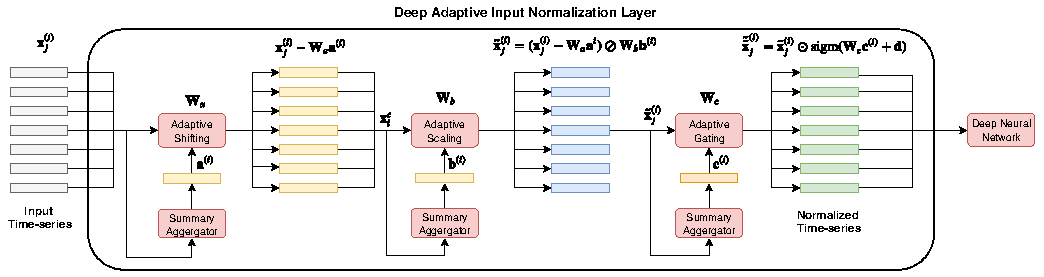
\includegraphics[width=\textwidth]{diagrams/dain_diagram.pdf}
\end{center}
\caption{Architecture of the \acf{DAIN} layer, proposed by \citeauthor{dain}. The diagram
is taken from page 2 of \citep{dain}.}
\label{fig:dain-arch}
\end{figure}


\subsubsection{RDAIN}%
\label{ssub:RDAIN}

The \ac{RDAIN} method is presented in \cite{rdain}.

\subsubsection{BiN}%
\label{ssub:BiN}

The \ac{BIN} layer is presented in \cite{bin}.

% }}}


% }}}

%%%%%%%%%%%%%%%%%%%%%%%%%%%%%%%%%%%%%%%%%%%%%%%%%
\chapter{Methods} %%%%       METHODS         %%%%
%%%%%%%%%%%%%%%%%%%%%%%%%%%%%%%%%%%%%%%%%%%%%%%%%

% Introduction
% Introduction {{{
In this chapter, I present three novel preprocessing methods. The first method, abbreviated
\acs{EDAIN}, is based on existing work by \citeauthor{dain} and \citeauthor{bin}. It
is an adaptive preprocessing method, so it performs a sequence of parametrised transformations
on the input data before passing it to a deep neural network. To optimize the adaptive layer, 
the deep
neural network is augmented with the \acs{EDAIN} layer and both the neural network parameters
and the \acs{EDAIN} parameters are trained with stochastic gradient descent.
In \cref{sec:EDAIN-KL-method}, I present the second method, abbreviated \acs{EDAIN-KL}.
This method uses a very similar architecture to the \acs{EDAIN} layer, but instead of fitting the
parameters using stochastic gradient descent, it is optimised with a technique inspired by
\textit{normalizing flow} networks. In \cref{sec:PREPMIX-CAPS-method}, my third
contribution, the \acs{PREPMIX-CAPS} procedure, is presented. This procedure is significantly
different from the first two methods, as it automatically selects a mixture of static preprocessing
techniques to apply to the data instead of using adaptive transformations.

% }}}

\section{EDAIN}% EDAIN
% Methods: EDAIN {{{
\label{sec:EDAIN-method}

% Topics of this section:
% * Illustrative diagram of the 4 layers, and the weights, justifying order of operations
% * Differences to DAIN, explaining batch awareness, and specifics of (amex) dataset worked with
% * Explaining the 3 parts:
%   * outlier removal: Inspired by winsorization, plot of curve for different values,to show how work
%   * scale&shift: able to generalise standard scaling
%   * power transform: should also work for negative and positive values, while being numerically stable


My first contribution is the \ac{EDAIN} layer. This adaptive preprocessing layer is inspired
by the likes of \citep{dain}  and \citep{bin}, but unlike the aforementioned methods, the
\ac{EDAIN} layer also supports normalizing the data in a \textit{global-aware} fashion, whereas
the \ac{DAIN}, \ac{RDAIN} and \ac{BIN} layers are all \textit{local-aware}.
The \ac{EDAIN} layer has four different sublayers. The first sublayer reduces the effect of
outliers in the data, while the second and third sublayer perform and adaptive shift and
scale operation. Finally, an adaptive power transform operation is applied to reduce the
skewness of the input data.

\subsection{Architecture}%
\label{sub:Architecture}

% Latex equations used:
% \(\mathbf{\alpha}' \odot \left(\mathbf{\beta}' \odot \tanh\left\{(\mathbf{x}_t^{(i)}-\hat{\mathbf\mu}) \oslash \mathbf{\beta}'  \right\}+\hat{\mathbf\mu} \right)+\left(1-\mathbf{\alpha}' \right) \odot \mathbf{x}_t^{(i)}\)
% \((\mathbf{\tilde{x}}_t^{(i)}  - \mathbf{\gamma} \mathbf{\mu}_{\mathbf{\tilde{x}}_t^{(i)}}) \oslash \mathbf{\lambda} \sigma_{\mathbf{\tilde{x}}_t^{(i)}}, \textrm{ if local-aware} \)
% TODO: add w=(alpha, beta) above the red boxes to highlight which parameters are optimized...
\begin{figure}
\begin{center}
    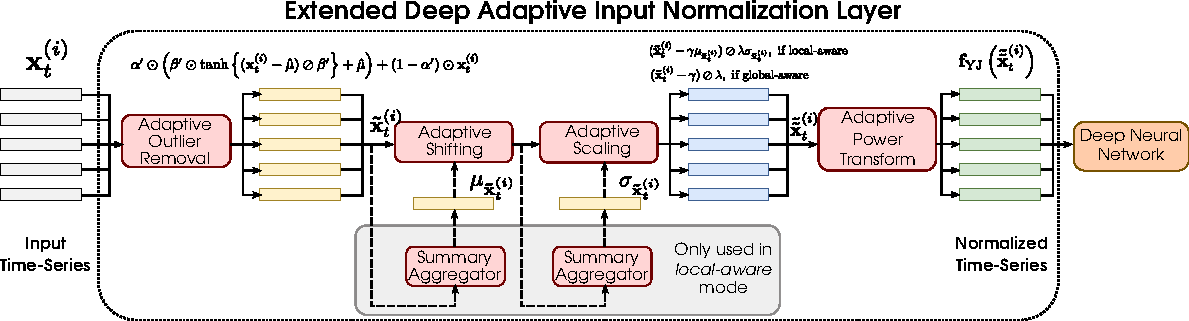
\includegraphics[width=\textwidth]{diagrams/edain-diagram.pdf}
\end{center}
\caption{An overview of the architecture of the proposed \ac{EDAIN} normalization layer.}
\label{fig:edain-arch}
\end{figure}

An overview of the layer's architecture is shown in figure \cref{fig:edain-arch}.
Given some input time-series $\bfX^{(i)} \in \R^{d \times T}$, each temporal segment
$\bfx^{(i)}_t$ is passed through an adaptive outlier removal layer, followed by an adaptive shift
and scale operation, and then finally passed through an adaptive power transformation layer.
The architecture also has two modes, \textit{local-aware} and \textit{global-aware}. In
global-aware mode, the \ac{EDAIN} layer aims to normalize each input such that the resulting
distribution of all the samples in the dataset resemble a unimodal normal distribution, that is,
a ``global normalization''. In local-aware mode,
the \ac{EDAIN} layer's normalization operations
also depend on summary statistics of each input sample $\bfX^{(i)}$, and the goal is to transform
all the data into a common normalized representation space, independent of where in the
``global distribution'' the sample originated from. This mode is most suitable for
multi-modal input data, as samples from different modes can all be transformed into one common
normalized unimodal distribution. On the other hand, the global-aware mode
is most suitable if all the data comes from a similar data generation mechanism,
and works best if the input data has few modes.
In local-aware mode, the \ac{EDAIN} architecture is similar to the
\ac{DAIN} architecture proposed by \citeauthor{dain} and shown
in \cref{fig:dain-arch}, but it
extends it with both a global-aware mode as well as an adaptive outlier removal sublayer and
an adaptive power transform sublayer.

% Outlier removal
\subsubsection{Outlier removal}% {{{
\label{ssub:Outlier removal}

Handling outliers and extreme values in the dataset can increase predictive performance if done
correctly (citation needed). Two common ways of doing this are omission and winsorization
\citep{winsorization}. With the former, observations that are deemed to be extreme are simply
removed during training. With the latter, all the data is still used, but observations lying
outside a certain number of standard deviation from the mean, or below or above certain
percentiles, are \textit{clipped} to be closer to the mean or median of the data. We refer to this
technique as \textit{winsorization}.
For example, if winsorizing data using 3 standard deviation, all values less than
$\mu-3\sigma$ are set to be exactly $\mu-3\sigma$. Similarly, the values above
$\mu+3\sigma$ are clipped to this value. Winsorization can also be done using percentiles,
where common boundaries are the first and fifth percentiles \citep{winsorization}.
However, the type of winsorization, as well as the number of standard deviation
or percentiles to use, might depend on the dataset. Additionally, it might not
be necessary to winsorize the data at all if the outliers turn out to not
negatively affect performance. All this introduces more hyperparameters to tune
during modelling. The outlier removal operation presented here aims to automatically  determine both
whether winsorization is necessary for a particular feature, and determine the threshold at
which to apply winsorization.

For input vector $\bfx_t^{(i)} \in \R^d$, the adaptive outlier removal operation is defined as:
\begin{equation}\label{eq:adaptive-outlier-removal}
    \mathbf{h}_1(\bfx_t^{(i)})=\bm\alpha' \odot \underbrace{\left(\bm\beta' \odot
        \tanh\left\{\left(\bfx_t^{(i)}-\hat{\bm\mu}\right) \oslash \bm\beta'  \right\}+\hat{\bm\mu}
\right)}_{\text{smooth adaptive centred winsorization}}
    +\underbrace{\left(1-\bm\alpha' \right) \odot \bfx}_{\text{residual connection}},
\end{equation}
where
$\bm\alpha' \in [0,1]^d$ is a parameter controlling how much winsorization to apply to each feature,
and $\bm\beta' \in [\beta_{\text{min}},\infty)^d$ controls the winsorization threshold for
each feature, that is, the maximum absolute value of the output, thus controlling the range of the
output. The effect of the two parameters is illustrated in \cref{fig:adaptive_outlier}.
The unknown parameters of the model are $\bm\alpha \in \R^d$ and $\bm\beta \in \R^d$, and they
are transformed into the constrained parameters $\bm\alpha'$ and $\bm\beta'$, as used in
\cref{eq:adaptive-outlier-removal} through the following  mappings:
\begin{equation}
    \bm\alpha'=\frac{e^{\bm\alpha}}{1\oplus e^{\bm\alpha}} \qquad\qquad
    \bm\beta'=\beta_{\text{min}}\oplus e^{\bm\beta},
\end{equation}
where $\beta_{\textrm{min}} \in \R$ is a hyperparameter that can be tuned, but a suitable value is $\beta_{\textrm{min}}=1$. We introduce $\beta_{\textrm{min}}>0$ to prevent the sublayer from
squeezing all the data into the range $[0,0]$ during training, as the smallest possible range
with the parameter becomes $[-\beta_{\textrm{min}}, \beta_{\textrm{min}}]$.


The $\hat{\bm\mu}\in \R^d$ parameter in \cref{eq:adaptive-outlier-removal} is an estimate of the mean of the data, and is used
to ensure the winsorization is centred. When setting the \ac{EDAIN} layer in \textit{local-aware}
mode, it is simply the mean of the current batch of data points, $\mathcal{B}$:
\begin{equation}
    \hat{\mu}_k=\frac{1}{|\mathcal{B}| T} \sum_{i \in \mathcal{B}} \sum_{t=1}^T x_{t,k}^{(i)}, \qquad k=1,\dots,d.
\end{equation}
In \textit{global-aware} mode, it is iteratively updated using a \textit{cumulative
moving average estimate} at each forward pass of the sublayer.
This is to better approximate the global mean of the data.
% For ease of notation, we let $\mathbf{W}_1=(\bm\alpha, \bm\beta)$ denote the $2d$ unknown
% parameters that are optimised for the adaptive outlier removal layer.

\begin{figure}
\begin{center}
    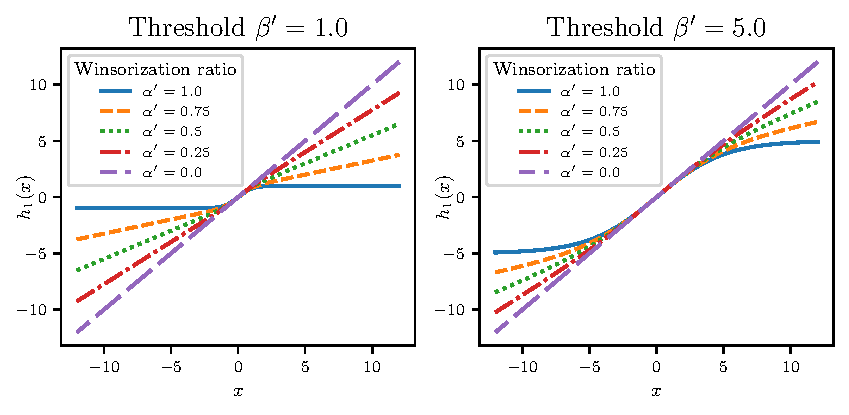
\includegraphics[scale=1.0]{figures/adaptive_outlier_removal.pdf}
\end{center}
\caption{Plot of the adaptive outlier removal operation for different combinations of parameter
values for $\alpha'$ and $\beta'$.}
\label{fig:adaptive_outlier}
\end{figure}


% }}}

% Scale and shift
\subsubsection{Scale and shift}% {{{
\label{ssub:Scale and shift}

Depending on the dataset, one might want to aim for a \textit{global
normalization}, in which case a \textit{global-aware} scale and shift operation is most
suitable. If the dataset has many different modes, with significantly different distribution characteristics, a \textit{local normalization} based on the specific mode each data point comes from is more suitable, in which case a \textit{local-ware} scale and shift
operation works best. This gives two different approaches and scaling and shifting the data in an adaptive fashion.

\paragraph{Global-aware}%
\label{par:Global-aware}

In global-aware mode, the adaptive shift and scale layer, combined, simply performs the operation
\begin{equation}\label{eq:adaptive-scale-shift}
    \mathbf{h}_3(\mathbf{h}_2(\bfx_t^{(i)})):=(\bfx_t^{(i)} - \bm\gamma) \oslash \bm\lambda,
\end{equation}
where the unknown parameters are $\bm\gamma \in \R^d$ and $\bm\lambda \in (0,\infty)^d$.
This makes the scale-and-shift layer a generalised version of
Z-score scaling, or standard scaling, as setting
\begin{equation}
    \bm\gamma:=\frac{1}{N T}  \sum^{N}_{i=1} \sum^{T}_{t=1} \bfx_{t}^{(i)}
\end{equation}
and
\begin{equation}
    \bm\lambda:=\frac{1}{N T} \sum^{N}_{i=1} \sum^{T}_{t=1} \left(\bfx_{t}^{(i)}- \bm\gamma\right)^2
\end{equation}
makes the operation in \cref{eq:adaptive-scale-shift} equivalent to Z-score scaling.
This \textit{global-aware} mode is useful if the distribution is similar across batches
and constitute a global unimodal distribution that should be centred, as the operation can generalise Z-score scaling.

\paragraph{Local-aware}%
\label{par:Local-aware}

Some datasets might have multiple modes arising from significantly different
data generation mechanisms. Attempting to scale and shift each batch to a global mean and
standard deviation might hurt performance in such cases. Instead, \citeauthor{dain} propose
basing the scale and shift on a \textit{summary representation} of each data point, allowing
each sample to be normalized according the specific mode  of the data it originated from.
This gives
\begin{equation}
    \mathbf{h}_3\left(\mathbf{h}_2\left(\bfx_t^{(i)}\right)\right):= 
    \left(\bfx_t^{(i)} - \left[\bm\gamma \odot \mu_{\bfx}^{(i)}\right]\right) \oslash \left[\bm\lambda \odot \sigma_{\bfx}^{(i)}\right],
\end{equation}
where the summary representations $\sigma_{\bfx}^{(i)} \in \R^d$ and $\mu_{\bfx}^{(i)} \in \R^d$ are computed through a reduction
along the temporal dimension of each observation:
\begin{align}
    \mu_\bfx^{(i)}&=\frac{1}{T} \sum^{T}_{t=1} \bfx^{(i)}_t  \\
    \sigma_\bfx^{(i)}&=\sqrt{\frac{1}{T}  \sum^{T}_{t=1} \left(\bfx^{(i)}_t- \mu_\bfx^{(i)} \right)^2}.
\end{align}
With this mode, it is difficult for the layer to generalise Z-score scaling, but it allows
discarding mode information such that highly multimodal distributions appear unimodal after passing
through the layer.

% }}}

% Power transform
\subsubsection{Power transform}% {{{
\label{ssub:Power transform}

Many real-world datasets exhibit significant skewness, which is often treated using power
transformations (citation needed). The most common transformation is the Box-Cox transformation,
but this is only valid for positive values, so it is not applicable to most real-world datasets
\citep{boxcox}. An alternative is a transformation proposed by \citeauthor{yeoJohnson},
known as the Yeo-Johnson transform:
\begin{equation}\label{eq:yeo-johnson}
    f_{\textrm{YJ}}^\lambda(x)= \left\{
        \begin{array}{ll}
            \frac{(x+1)^{\lambda}-1}{\lambda}, & \textrm{if } \lambda \neq 0, x \geq 0; \\
            \log(x + 1), & \textrm{if } \lambda = 0, x \geq 0;  \\
            \frac{(1-x)^{2-\lambda}-1}{\lambda-2} , & \textrm{if } \lambda \neq 2, x < 0; \\
            -\log(1-x), & \textrm{if } \lambda=2, x < 0.
        \end{array}
    \right.
\end{equation}
Like the Box-Cox transformation, the transformation $f_{\textrm{YJ}}$ only has one unknown parameter, $\lambda$, but
it works for any $x \in \R$, not just positive values \citep{yeoJohnson}.
The power transform layer simply applies the transformation in \cref{eq:yeo-johnson} along each dimension of the input, that is for each $i=1,\dots,N$ and $t=1,\dots,T$,
\begin{equation}
    \left[\mathbf{h}_4\left(\bfx_t^{(i)}\right)\right]_j:=f^{\lambda_j^{(\textrm{YJ})}}_{\textrm{YJ}}\left(x_{t,j}^{(i)}\right), \;\;\; j=1,\dots,d.
\end{equation}
The vector of the $d$ unknown parameter for the Yeo-Johnson transformation will be
denoted $\bm\lambda^{(\textrm{YJ})} \in \R^d$, as to not be confused with the scale parameter
$\bm\lambda \in \R^d$.


% }}}

% Optimising the parameters
\subsection{Optimisation through stochastic gradient descent}% {{{
\label{sub:Optimising the parameters}

To optimise the unknown parameters
$\left( \bm{\alpha}, \bm{\beta}, \bm{\gamma}, \bm{\lambda}, \bm{\lambda}^{(\textrm{YJ})}\right)$,
the deep neural network is augmented by prepending the \ac{EDAIN} layer, as shown in
\cref{fig:edain-arch}. Then the input data is fed into the augmented model in batches,
as when training a neural network, and after each forward pass of the model, the weights
are updated through stochastic gradient descent while training the neural network.
As observed by \citeauthor{dain}, the model convergence is unstable if the same learning rate
$\eta \in \R$ that is used for training the deep neural network is also used for training all
the sublayers of the \ac{EDAIN} layer. Therefore, separate learning rate modifiers
$\eta_{\textrm{out}}$,
$\eta_{\textrm{shift}}$,
$\eta_{\textrm{scale}}$ and
$\eta_{\textrm{pow}}$ for the outlier removal, shift, scale and power transform sublayers are
introduced as additional hyperparameters and the weight updates happen according to the equation:
\begin{equation}
    \Delta \left( \bm{\alpha}, \bm{\beta}, \bm{\gamma}, \bm{\lambda}, \bm{\lambda}^{(\textrm{YJ})}\right)
    =
    -\eta\left(
        \eta_{\textrm{out}} \frac{\partial \mathcal{L}}{\partial \bm\alpha},
        \eta_{\textrm{out}} \frac{\partial \mathcal{L}}{\partial \bm\beta},
        \eta_{\textrm{shift}} \frac{\partial \mathcal{L}}{\partial \bm\gamma},
        \eta_{\textrm{scale}} \frac{\partial \mathcal{L}}{\partial \bm\lambda},
        \eta_{\textrm{pow}} \frac{\partial \mathcal{L}}{\partial \bm{\lambda}^{(\textrm{YJ})}}
    \right),
\end{equation}
where $\mathcal{L}$ denotes the criterion evaluated at a batch of inputs and targets.


% }}}

% }}}

\section{EDAIN-KL}% EDAIN-KL
% Methods: EDAIN-KL {{{
\label{sec:EDAIN-KL-method}

The \ac{EDAIN-KL} layer has a very similar architecture to the earlier-presented
\ac{EDAIN} layer, but the unknown parameter are optimised in a completely different
manner. Unlike the \ac{EDAIN} layer, the \ac{EDAIN-KL} layer is not attached to the deep neural
network during training and thus not trained simultaneously with the neural network. Instead,
before training the neural network, we train the \ac{EDAIN-KL} layer in isolation.
This is done by using it to transform a standard
normal distribution into a distribution that is similar to our training dataset. Then, after
the \ac{EDAIN-KL} weights have been optimized, we use the layer in reverse to normalize samples
from the training dataset before passing it to the neural network.

\subsection{Architecture}%
\label{sub:Architecture}

The \ac{EDAIN-KL} layer has a very similar architecture to the \ac{EDAIN} layer, described in
\cref{sec:EDAIN-method}, but the outlier removal transformation has been simplified to ensure its
inverse is analytic. Additionally, the layer no longer supports local-aware mode, as this
would make the inverse intractable. The \ac{EDAIN-KL} transformations are:
\begin{align}
    \textrm{(Outlier removal)} \qquad& \mathbf{h}_1\left(\bfx^{(i)}_t\right)=\bm\beta' \odot \tanh\left\{(\bfx^{(i)}_t - \hat{\bm\mu}) \oslash \bm\beta' \right\}+\hat{\bm\mu} \label{eq:kl1}\\
    \textrm{(shift)} \qquad& \mathbf{h}_2\left(\bfx^{(i)}_t\right)=\bfx^{(i)}_t- \bm\gamma \label{eq:kl2}\\
    \textrm{(scale)} \qquad& \mathbf{h}_3\left(\bfx^{(i)}_t\right)=\bfx^{(i)}_t \oslash \bm\lambda  \label{eq:kl3}\\
    \textrm{(power transform)} \qquad& \mathbf{h}_4\left(\bfx^{(i)}_t\right)=\left[
        f^{\lambda_1^ {(\textrm{YJ})} }_{\textrm{YJ}}\left(x^{(i)}_{t,1}\right)
        % \quad f^{\lambda_2^ {(\textrm{YJ})}}_{\textrm{YJ}}\left(x^{(i)}_{t,1}\right)
        \quad \cdots
        \quad f^{\lambda_d^ {(\textrm{YJ})}}_{\textrm{YJ}}\left(x^{(i)}_{t,d}\right)
    \right], \label{eq:kl4}
\end{align}
where $f^{\lambda_i^ {(\textrm{YJ})}}_{\textrm{YJ}}(\cdot)$ is defined in \cref{eq:yeo-johnson}.

\subsection{Optimisation through Kullback-Leibler divergence}%
\label{sub:Optimisation through Kullback-Leibler divergence}

The  optimisation approach used to train the \ac{EDAIN-KL} method is inspired by normalizing flow,
of which \citeauthor{normalizing_flows} provide a great overview of \cite{normalizing_flows}.
Before describing the approach, we provide a brief overview of related notation and some
background on the concept behind normalizing flows. After this, we go through how the
\ac{EDAIN-KL} layer itself can be treated as an invertible bijector to fit into the
normalizing flow framework. In doing so, we realize the need for analytic and differentiable
expressions for certain terms related to the \ac{EDAIN-KL} layer. Derivations for these terms are
then presented.

\subsubsection{Brief background on normalizing flow}%
\label{ssub:Brief background on normalizing flow}

The idea behind normalizing flow is taking a simple random variable, such as a standard
Gaussian, and transforming it into a more complicated distribution, for example, one that
resembles the distribution of a given dataset of samples.
Consider a random variable $\bfZ \in \R^d$ with a known and
analytic expression for the \ac{pdf} $p_\bfz: \R^d \rightarrow {\R}$. We refer to $\bfZ$ as
the \textit{base distribution}. We then define
a parametrised invertible function
$\mathbf{g}_{\bm \theta}:\R^d \rightarrow {\R^d}$, also known as a \textit{bijector},
and use this to transform the base distribution into a new
 probability distribution: $\bfY=\mathbf{g}_{\bm\theta}(\bfZ)$.
By increasing the complexity of the bijector $\mathbf{g}_{\bm\theta}$, by for instance using
a deep neural network, the transformed distribution $\bfY$ can grow arbitrarily complex as well.
The \ac{pdf} of the transformed distribution can then be computed using the change of variable
formula \citep{normalizing_flows}, where
\begin{align}
    p_\bfY(\bfy)&=p_\bfZ(\mathbf{g}_{\bm\theta}^{-1}\left(\bfy\right))\cdot \left|\det \mathbf{J}_{\bfY \rightarrow {\bfZ}}\left(\bfy \right) \right| \nonumber \\
                & = p_\bfZ(\mathbf{g}_{\bm\theta}^{-1}\left(\bfy\right))\cdot \left|\det \mathbf{J}_{\bfZ \rightarrow {\bfY}}\left( \mathbf{g}^{-1}_{\bm\theta}(\bfy) \right) \right|^{-1}, \label{eq:sj98days9dohao}
\end{align}
where $\mathbf{J}_{\bfZ \rightarrow {\bfY}}$ is the Jacobian matrix for the \textit{forward mapping}
$\mathbf{g}_{\bm\theta} : \bfz \mapsto \bfy$. Recall
that the $(i,j)$th entry of the Jacobian matrix of some multivariate function $\mathbf{f}$ is
given by $\mathbf{J}_{ij}=\frac{\partial f_i}{\partial x_j}$.
Taking logs on both sides of \cref{eq:sj98days9dohao}, it follows that
\begin{equation}\label{eq:logDetJac}
    \log p_\bfY(\bfy)= \log p_\bfZ(\mathbf{g}_{\bm\theta}^{-1}\left(\bfy\right)) - \log \left|\det \mathbf{J}_{\bfZ \rightarrow {\bfY}}\left(\mathbf{g}_{\bm\theta}^{-1}\left(\bfy\right) \right) \right|.
\end{equation}

One common application of normalizing flows is density estimation \citep{normalizing_flows};
Given a dataset $\mathcal{D}=\{\bfy^{(i)}\}_{i=1}^N$ with samples from some
unknown, complicated distribution, we want to estimate its \ac{pdf}.
This can be done with likelihood-based estimation, where we assume the data points
$\bfy^{(1)}, \bfy^{(2)},\dots,\bfy^{(N)}$ come from, say,
the parametrised distribution $\bfY=\mathbf{g}_{\bm \theta}(\bfZ)$ and
we optimise $\bm\theta$ to maximise the data log-likelihood,
\begin{align}
    \log p(\mathcal{D}| \bm\theta)
    & = \sum_{i=1}^N \log p_\bfY(\bfy^{(i)}| \bm\theta ) \\
    &\stackrel{\cref{eq:logDetJac}}{=} \sum^{N}_{i=1}
    \log p_\bfZ\left(\mathbf{g}_{\bm\theta}^{-1}\left(\bfy^{(i)}\right)\right) - \log \left|\det \mathbf{J}_{\bfZ \rightarrow {\bfY}}\left(\mathbf{g}_{\bm\theta}^{-1}\left(\bfy^{(i)}\right)\right) \right|. \label{eq:logProbKL}
\end{align}
This is equivalent to minimising the \ac{KL-divergence} between the empirical distribution
$\mathcal{D}$ and the transformed distribution $\bfY=\mathbf{g}_{\bm\theta}(\bfZ)$:
\begin{align}
    \argmax_{\bm\theta} \log p(\mathcal{D}| \bm\theta)
    &= \argmax_{\bm\theta}\sum_{i=1}^N \log p_\bfY \left(\bfy^{(i)}\big|\bm\theta \right) \\
    &=\frac{1}{N}  \sum_{i=1}^N \log p_{\mathcal{D}}\left(\bfy^{(i)}\right)
        +\argmax_{\bm\theta}\frac{1}{N} \sum_{i=1}^N \log p_\bfY \left(\bfy^{(i)}\big|\bm\theta \right) \\
    &= \argmin_{\bm\theta}\frac{1}{N}  \sum_{i=1}^N \log p_{\mathcal{D}}\left(\bfy^{(i)}\right)
    -\frac{1}{N} \sum_{i=1}^N \log p_\bfY \left(\bfy^{(i)}\big|\bm\theta \right) \\
    &= \argmin_{\bm\theta}\sum^{N}_{i=1}  p_\mathcal{D}\left(\bfy^{(i)}\right)  \log p_{\mathcal{D}}\left(\bfy^{(i)}\right) \\
    &\qquad- \sum_{i=1}^N  p_\mathcal{D}\left(\bfy^{(i)}\right) \log p_\bfY \left(\bfy^{(i)}\big|\bm\theta \right) \\
    &= \argmin_{\bm\theta} D_{\textrm{KL}}\left(\mathcal{D}\;||\; (\bfY\mid\bm\theta)\right).
\end{align}
When training an normalizing flow model, we want to find the parameter values
$\bm\theta$ that minimize the above \ac{KL-divergence}.
This is done using stochastic gradient descent and backpropagation, as described in
\cref{sec:Deep learning} where the criterion $\mathcal{L}$ is set to be the negation
of \cref{eq:logProbKL}. That is, the loss becomes the negative log likelihood of a batch
of samples from the training dataset. To perform optimisation with this criterion,
we need to compute all the terms in \cref{eq:logProbKL} and this expression needs to
be differentiable, as the backpropagation algorithm uses the gradient of the loss
with respect to the input data.
We therefore need to find
\begin{enumerate}[(i)]
    \item  an analytic and differentiable expression for the inverse transformation
$\mathbf{g}_{\bm\theta}^{-1}\left(\cdot \right)$,
    \item  an analytic and differentiable expression for the \ac{pdf} of the base distribution
$p_{\bfZ}(\cdot)$, and
    \item an analytic and differentiable expression for the log determinant of the Jacobian matrix for $\mathbf{g}_{\bm\theta}$, that is
$\log \left|\det \mathbf{J}_{\bfZ \rightarrow {\bfY}} \right|$.
\end{enumerate}
We will derive these three components for our \ac{EDAIN-KL} layer in the next section, but
before doing that, we make note of the following lemma.
Using a result stated in \citeauthor{normalizing_flows}, the following can be shown:
\begin{lemma}\label{thrm:normFlow}
    Let $\mathbf{g}_1,\dots, \mathbf{g}_n:\R^d \rightarrow {\R^d}$ all be bijective functions, and consider
    the composition of these functions, $\mathbf{g}=\mathbf{g}_n \circ \mathbf{g}_{n-1} \cdots \circ \mathbf{g}_1$.
    Then, $\mathbf{g}$ is a bijective function with inverse
    \begin{equation}
        \mathbf{g}^{-1}=\mathbf{g}_1^{-1} \circ \cdots \circ \mathbf{g}_{n-1}^{-1} \circ \mathbf{g}_n^{-1},
    \end{equation}
    and the log of the absolute value of the determinant of the Jacobian is given by
    \begin{equation}
        \log \left| \det \mathbf{J}_{\mathbf{g}^{-1}}(\cdot)\right|
        = \sum_{i=1}^N \log\left|\det \mathbf{J}_{\mathbf{g}_i^{-1}}(\cdot) \right|.
    \end{equation}
    Similarly,
    \begin{equation}
        \log \left| \det \mathbf{J}_{\mathbf{g}}(\cdot)\right|
        = \sum_{i=1}^N \log \left|\det \mathbf{J}_{\mathbf{g}_i}(\cdot) \right|.
    \end{equation}
\end{lemma}

\subsubsection{Application to EDAIN-KL}%
\label{ssub:Application to EDAIN-KL}

Like with the \ac{EDAIN} layer, we want to compose the outlier removal, shift, scale and power
transform transformations into one operation, which we do by defining
\begin{equation}\label{eq:gtheta}
    \mathbf{g}_{\bm\theta}=\mathbf{h}_1^{-1} \circ  \mathbf{h}_2^{-1} \circ \mathbf{h}_3^{-1} \circ \mathbf{h}_4^{-1},
\end{equation}
where $\bm\theta=(\bm\beta, \bm\gamma, \bm\lambda, \bm\lambda^{(\textrm{YJ})})$ and
$\mathbf{h}_1,\dots,\mathbf{h}_4$ are defined in \cref{eq:kl1,eq:kl2,eq:kl3,eq:kl4}, respectively.
Notice that we apply all the operations in reverse order, compared to the \ac{EDAIN} layer. This
is because we will use $\mathbf{g}_{\bm\theta}$ to transform our base distribution $\bfZ$ into
a distribution that resembles the training dataset, $\mathcal{D}$, not the other way around.
Then, to normalize the dataset after fitting the \ac{EDAIN-KL} layer, we apply
\begin{equation}\label{eq:gthetainv}
    \mathbf{g}_{\bm\theta}^{-1}=\mathbf{h}_4 \circ \mathbf{h}_3 \circ \mathbf{h}_2 \circ \mathbf{h}_1
\end{equation}
to each sample, similar to the \ac{EDAIN} layer.
It can be shown that all the transformations defined in
\cref{eq:kl1,eq:kl2,eq:kl3,eq:kl4} are invertible, of which a proof is given in
the next subsection.
Using \cref{thrm:normFlow}, it thus follows that
$\mathbf{g}_{\bm\theta}$, as defined in \cref{eq:gtheta}, is bijective and that its inverse
is given by \cref{eq:gthetainv}. Noticing that we already have analytic and differentiable
expressions for $\mathbf{h}_1$, $\mathbf{h}_2$, $\mathbf{h}_3$, $\mathbf{h}_4$ in
\cref{eq:kl1,eq:kl2,eq:kl3,eq:kl4}, the inverse of the bijector, $\mathbf{g}_{\bm\theta}^{-1}$,
defined in \cref{eq:gthetainv} also has an analytic and differentiable expression, so part
(i) is satisfied.

We now move onto deciding what our base distribution should be.
Making the input data as Gaussian as possible usually increases performance of deep sequence models
(citation needed), so a suitable base distribution is the standard multivariate Gaussian distribution
\begin{equation}
    \bfZ \sim \mathcal{N}(0, \mathbf{I}_d),
\end{equation}
whose \ac{pdf} $p_\bfZ(\cdot)$
has a nice analytic and differentiable expression, so part $(\textrm{ii})$ is satisfied.

In order to optimise the unknown parameters
$\bm\theta=(\bm\beta, \bm\gamma, \bm\lambda, \bm\lambda^{(\textrm{YJ})})$ of the
\ac{EDAIN-KL} layer by treating it as a normalizing flow bijector, we need an analytic and
differentiable expression for the right-hand side of \cref{eq:logProbKL}. We already have
an expression for part (i) and part (ii), so only part  (iii) remains.
That is, an analytic and differentiable expression for
the log of the determinant of the Jacobian matrix of $\mathbf{g}_{\bm\theta}$, $\log\left|\det \mathbf{J}_{\bfZ \rightarrow {\bfY}} \right|$. We will derive this
in the next subsection. Once that is done, parts (i), (ii) and (iii) are satisfied, so
$\bm\theta$ can be optimised using back-propagation as described in \cref{sec:Deep learning},
using the negation of \cref{eq:logProbKL} as the objective. In other words, we can optimise
$\bm\theta$ to maximise the likelihood of the training data under the assumption that it comes from
the distribution $\bfY= \mathbf{g}_{\bm\theta}(\bfZ)$. This is desirable, as if we can achieve
a high data likelihood, the samples $\bfy$ will more closely resemble a standard normal distribution
after being transformed by $\mathbf{g}_{\bm\theta}^{-1}$ after fitting the bijector.
This might then increase the performance as the neural network will be fed data
that is more Gaussian.

\subsubsection{Derivation
of %$\mathbf{g}_{\bm\theta}^{-1}$ and
$\log \left|\det \mathbf{J}_{\bfZ \rightarrow {\bfX}}\right|$}%
\label{ssub:ildj}

Recall that the \ac{EDAIN-KL} architecture is just a bijector that is composed of 4 other bijective
functions. Using the result in \cref{thrm:normFlow}, we get
\begin{equation}
    \log \left|\det \mathbf{J}_{\bfZ \rightarrow {\bfY}}(\cdot)  \right|
    = \sum^{4}_{i=1} \log \left|\det \mathbf{J}_{\mathbf{h}_i^{-1}}(\cdot) \right|.
\end{equation}
Considering the transformations in \cref{eq:kl1,eq:kl2,eq:kl3,eq:kl4}, we notice that all the
transformation happen element-wise, so for $i\in\{1,2,3,4\}$, we have
$\left[\frac{\partial \mathbf{h}_i^{-1}(\bfx)}{\partial x_{k}}\right]_j =0$ for $k \neq j$.
Therefore, the Jacobians are diagonal matrices, so the determinant is just the product of the
diagonal entries, giving
\begin{align}
    \log \left|\det \mathbf{J}_{\bfZ \rightarrow {\bfY}}(\bfx)  \right|
    & = \sum^{4}_{i=1} \log \left| \prod_{j=1}^d \left[\frac{\partial \mathbf{h}_i^{-1}(\bfx)}{\partial x_j}\right]_j   \right| \\
    & = \sum^{4}_{i=1} \sum_{j=1}^d \log \left| \left|\frac{\partial \mathbf{h}_i^{-1}(\bfx)}{\partial x_j}\right|_j   \right| \\
    & = \sum^{4}_{i=1} \sum_{j=1}^d \log \left| \frac{\partial h_i^{-1}\left(x_j;\theta_j^{(i)}\right)}{\partial x_j}  \right|, \label{eq:sgas9fg8a9sd8}
\end{align}
where in the last step we used the fact that $h_1,h_2,h_3$ and $h_4$ are applied element-wise
to introduce the notation $h_i(x_j;\theta^{(i)}_j)$ that means applying $\mathbf{h}_i$ to
some vector where the $j$th element is $x_j$, and the corresponding $j$th transformation
parameter takes the value $\theta^{(i)}_j$. For example, for the scale
function, $\mathbf{h}_3(\bfx)=\bfx \oslash \bm\lambda$, we have
$h_3(x_j;\lambda_j)=\frac{x_j}{\lambda_j}$.
From \cref{eq:sgas9fg8a9sd8}, we know that we only need to derive the derivatives for
the element-wise inverses, which we will now do for each of the four transformations.
In doing so, we also demonstrate that each transformation is bijective.

\paragraph{Shift}%
\label{par:Shift}

We first consider $h_2(x_j;\gamma_j)=x_j-\gamma_j$. Its inverse is $h_2^{-1}(z_j;\gamma_j)=z_j+\gamma_j$, and it follows that
\begin{equation}
    \log \left|\frac{\partial h_2^{-1}(z_j ; \gamma_j)}{\partial z_j} \right|
    = \log 1 = 0.
\end{equation}

\paragraph{Scale}%
\label{par:Scale}

We now consider $h_3(x_j;\lambda_j)=\frac{x_j}{\lambda_j}$, whose inverse is $h_3^{-1}(x_j;\lambda_j)={z_j}{\lambda_j}$. It follows that
\begin{equation}
    \log \left|\frac{\partial h_3^{-1}(z_j ; \gamma_j)}{\partial z_j} \right|
    = \log \left|{\lambda_j}  \right|.
\end{equation}

\paragraph{Outlier removal}%
\label{par:Outlier removal}

We now consider $h_1(x_j;\beta'_j)= \beta'_j \tanh\left\{\frac{(x_j - \hat{\mu}_j)}{\beta'_j}  \right\} + \hat{\mu}_j$. Its inverse is
\begin{equation}
    h_1^{-1}(z_j;\beta_j') =\beta' \tanh^{-1} \left\{\frac{z_j - \hat{\mu}_j}{\beta'_j}  \right\}
    +\hat{\mu}_j.
\end{equation}
It follows that
\begin{equation}
    \log \left|\frac{\partial h_1^{-1}(z_j ; \beta_j')}{\partial z_j} \right|
    = \log \left| \frac{1}{1-\left( \frac{z_j-\hat{\mu}_j}{\beta_j'}  \right)^2}  \right|
    = -\log\left| 1-\left( \frac{z_j-\hat{\mu}_j}{\beta_j'}  \right)^2 \right|.
\end{equation}

\paragraph{Power transform}%
\label{par:Power transform}

By considering the expression in \cref{eq:kl4}, it can be shown that for fixed
$\lambda^{(\textrm{YJ})}$, negative inputs are always
mapped to negative values and vice versa, which makes the Yeo-Johnson transformation invertible.
Additionally, in $\mathbf{h}_4(\cdot)$ the Yeo-Johnson transformation is applied element-wise, so
we get
\begin{equation}
    \mathbf{h}_4^{-1}(\mathbf{z})=\left[
        \left[f_{\textrm{YJ}}^{\lambda_1^{(\textrm{YJ})}}\right]^{-1}\bigg(z_1\bigg) \quad
        \left[f_{\textrm{YJ}}^{\lambda_2^{(\textrm{YJ})}}\right]^{-1}\bigg(z_2\bigg) \quad \cdots \quad
    \left[f_{\textrm{YJ}}^{\lambda_d^{(\textrm{YJ})}}\right]^{-1}\bigg(z_d\bigg) \right],
\end{equation}
where it can be shown that the inverse Yeo-Johnson transformation for a single element is given by
\begin{equation}
    \left[f_{\textrm{YJ}}^\lambda\right]^{-1}\bigg(z\bigg)= \left\{
    \begin{array}{ll}
        (z \lambda + 1)^{1/\lambda} -1, & \textrm{if } \lambda \neq 0, z \geq 0; \\
        e^z-1, & \textrm{if } \lambda = 0, z \geq 0;  \\
        1-\left\{1-z(2-\lambda)\right\}^{1/ (2-\lambda)} , & \textrm{if } \lambda \neq 2, z < 0; \\
        1-e^{-z}, & \textrm{if } \lambda=2, z < 0.
    \end{array}
    \right.
\end{equation}

The derivative with respect to $z$ then becomes
\begin{equation}
    \frac{\partial \left[f_{\textrm{YJ}}^\lambda\right]^{-1}(z)}{\partial z}= \left\{
        \begin{array}{ll}
            (z \lambda + 1)^{(1-\lambda)/\lambda}, & \textrm{if } \lambda \neq 0, z \geq 0; \\
            e^z, & \textrm{if } \lambda = 0, z \geq 0;  \\
            \left\{1-z(2-\lambda)\right\}^{(\lambda-1)/(2-\lambda)} , & \textrm{if } \lambda \neq 2, z < 0; \\
            e^{-z}, & \textrm{if } \lambda=2, z < 0.
        \end{array}
    \right.
\end{equation}
It follows that
\begin{equation}
    \log \left|\frac{\partial \left[f_{\textrm{YJ}}^\lambda\right]^{-1}(z)}{\partial z} \right|= \left\{
        \begin{array}{ll}
            \frac{1-\lambda}{\lambda}\log (z \lambda + 1), & \textrm{if } \lambda \neq 0, z \geq 0; \\
            z, & \textrm{if } \lambda = 0, z \geq 0;  \\
            \frac{\lambda - 1}{2-\lambda}\log\left\{1-z(2-\lambda)\right\} , & \textrm{if } \lambda \neq 2, z < 0; \\
            -z, & \textrm{if } \lambda=2, z < 0,
        \end{array}
    \right.
\end{equation}
which we use as the expression for $\log \left| \frac{\partial h_4^{-1}\left(z_j;\lambda_j^{(\textrm{YJ})}\right)}{\partial z_j} \right|$ for $z=z_1,\dots,z_d$.

Putting all of these expression together, we have an analytical and differentiable expression
for $\log\left| \det \mathbf{J}_{\bfZ \rightarrow {\bfY}}(\bfx) \right|$.

% TODO: write out the expression here.... ?

% }}}

\section{PREPMIX-CAPS}% PREPMIX-CAPS
% Methods: PREPMIX-CAPS {{{
\label{sec:PREPMIX-CAPS-method}

% TODO: find somewhere to mention this...
% Due to the computational complexity of the number of variables, the preprocessing of the
% multivariate time-series will be done \textit{across time}, that is, the same preprocessing method
% is applied to each of the variables, regardless of their timestep  index.


Unlike the \ac{EDAIN} and \ac{EDAIN-KL} layers, The \ac{PREPMIX-CAPS} procedure 
is not an adaptive preprocessing technique. Instead, it can be thought of as an automated way
of selecting the best static preprocessing technique for each predictor variable in the dataset.
Say we are working with multivariate time-series dataset where each time-series is of length $T$
and dimensionality $d$, that is, we have $d$ predictor variables.
The \ac{PREPMIX-CAPS} procedure starts with \textit{clustering phase},
producing $k$ clusters of the $d$ predictor variables,
where $k$ is a hyperparameter. There are two methods of clustering, one based on statistics
computed for each variable, and one based on the variables' relative \ac{KL-divergence}.
After the clustering has been performed, a static preprocessing method needs to be selected
for each cluster. This is done in an \textit{experiment running phase}. This phase has also
been  optimised with parallel computation, hence the ``parallel search'' in the procedure's
name.

\subsection{Clustering the predictor variables}%
\label{sub:prepmix-clustering}

We are working with a dataset of multivariate time-series,
$\mathcal{D}=\{\bfX^{(i)} \in \R^{d \times T}\}_{i=1,2,\dots,N}$.  In the
clustering phase, we want to determine how to segment the set of variables
$\{1,2,\dots,d\}$ into $k$ clusters such that the distribution of the
variables, according to $\mathcal{D}$, is as ``similar'' as possible within
each cluster.  The motivation behind this is that applying the same
preprocessing technique to similarly-distributed variables will have similar
effects on the neural network's performance, when trained on these preprocessed
variables.  To achieve a clustering where the distribution characteristics
within each clusters is as ``similar'' as possible, I propose two approaches:
Clustering based on distribution statistics, and an information theoretic clustering approach.

\subsubsection{Clustering based on statistics}%
\label{sub:Clustering based on statistics}

The first clustering approach is based on statistics. With this approach, we first compute
$d_{\textrm{stats}}$ different statistics for each of the $d$ predictor variables in the dataset $\mathcal{D}$.
This then gives a vector of $d_{\textrm{stats}}$ features for each of the $d$ predictor variables,
that can later be used as features in a clustering routine such as $K$-means. In this clustering
method, we have $d_{stats}=6$, and these statistics have been designed to quantitatively
capture a wide set of characteristics a distribution might have.

I will now present the six statistics that are computed
for each of the $d$ predictor variables.
The first statistic used is the Fisher's moment
coefficient of skewness \citep{shape}, which for $k=1,2,\dots,d$ is computed as
\begin{equation}\label{eq:fglkhy809s}
    \gamma_k=\frac{m_3}{m_2^{3/2}}, \quad \textrm{where }
    m_i=  \frac{1}{NT} \sum^{N}_{i=1} \sum^{T}_{t=1} \left(x^{(i)}_{t,k}-\mu_k \right)^i,
\end{equation}
where $\bm{\mu}=\frac{1}{NT}\sum^{N}_{i=1} \sum^{T}_{t=1} \bfx^{(i)}_t \in \R^d$ is the mean along the dimension-axis. 
The second statistic used is the kurtosis \citep{shape}, which for $k=1,2,\dots,d$ is computed as
\begin{equation}
    \alpha_k=\frac{m_4}{m_2^2},
\end{equation}
where $m_i$ for $i\in \{2,4\}$ is defined in  \cref{eq:fglkhy809s}.
The third statistic used is the standard deviation, computed as
\begin{equation}
    \sigma_k=\sqrt{m_2},
\end{equation}
where $m_2$ is defined in \cref{eq:fglkhy809s}.

% Binning statistics
The next three statistics are designed to capture characteristic of the variables' \ac{pdf}, but
since this is unknown, we approximate it by \textit{binning} the samples in the dataset
$\mathcal{D}$ in $n_{\textrm{num. bins}}$ distinct bins for each variable $k=1,2,\dots,d$.
We note that is done after applying Min-Max scaling on the dataset so that all the samples take
values in the range $[0,1]$.
Then consider $\mathbf{B} \in \R^{d \times \textrm{num. bins}}$,
where $B_{k,m}$ denotes the number of samples from the set of values corresponding to the
$k$th predictor, that is $\left\{x_{t,k}^{(i)} \right\}_{i=1,\dots,N,\;t=1,\dots,T}$,
that fall into the $m$th bin.
After performing this binning operation to get $\mathbf{B}$, the fourth statistic is computed as
\begin{equation}
    \frac{1}{n_{\textrm{num. bins} }}  \argmax_{i} B_{k,i},
\end{equation}
which approximates the normalized location of the highest mode in the variable's \ac{pdf}.
The fifth static is computed as
\begin{equation}
    \frac{1}{n_{\textrm{num. bins} }}  \sum^{n_{\textrm{num. bins} }}_{i=1} \mathbb{I}\left\{
        B_{k,i} > 0
    \right\},
\end{equation}
approximating how many unique values the distribution has. The sixth statistic is computed as
\begin{equation}
     \max_{i} B_{k,i},
\end{equation}
denoting the density in the highest mode in the \ac{pdf}.
After computing all the statistics and compiling the matrix
$\bfX' \in \R^{d \times d_{\textrm{stats} }}$ where the rows are feature vectors corresponding
to each predictor variable, we apply $K$-means clustering to get $k$ clusters
of the $d$ predictor \citep{kmeans}. However, before doing this, we perform Z-score scaling
on $\bfX'$ to ensure all the $d_{\textrm{stats}}$ are equally weighted in the clustering
routine.

\subsubsection{Clustering based on KL-divergence}%
\label{sub:Clustering based on KL-divergence}

The second clustering method is based on information theory.
One approach to putting ``similar'' variables in the same cluster is to cluster based on the
relative \ac{KL-divergence} between each variable.
To do this, we start by constructing a
distance matrix $\mathbf{W} \in \R^{d \times d}$ where $W_{i,j}$ denotes the
\ac{KL-divergence} between variable $X_j$ and $X_i$ for $j > i$. From
\citep{mackay} we can compute the \ac{KL-divergence} between predictor variable $X_j$ and $X_i$
with
\begin{equation}
    W_{i,j}= \sum^{n_{\textrm{num. bins} }}_{k=1} \mathbb{P}_{X_i}\left( \frac{k}{n_{\textrm{num. bins} }}  \right)
    \log\left\{
    \mathbb{P}_{X_i}\left( \frac{k}{n_{\textrm{num. bins} }}  \right) \bigg/
    \mathbb{P}_{X_j}\left( \frac{k}{n_{\textrm{num. bins} }}  \right)
\right\},
\end{equation}
where $\mathbb{P}_{X_i}(\cdot)$ is an approximation of the \ac{pdf} of the $i$th predictor variable.
We get this approximation by binning the samples after performing Min-Max normalization to ensure
the samples all fall in the range $[0,1]$, as was done when clustering based on statistics.
The integer $n_{\textrm{num. bins}}$ denote the number of bins used when doing this.
This distance matrix $\mathbf{W}$ is then used together with an \textit{agglomerative clustering}
approach to cluster the $d$ variables into $k$ clusters
\citep{hierarchical_clustering}. Since the distance matrix $\mathbf{W}$ is
non-Euclidean, the linkage criteria used was selected to be ``average''.

% TODO: does the reader really know what linkage criteria and anglomerative clustering is????

\subsection{Determining the optimal preprocessing method for each cluster}%
\label{sub:Determining the optimal preprocessing method for each clusterch cluster}

\begin{figure}[htp]
    \vspace*{-15pt}
    \begin{center}
        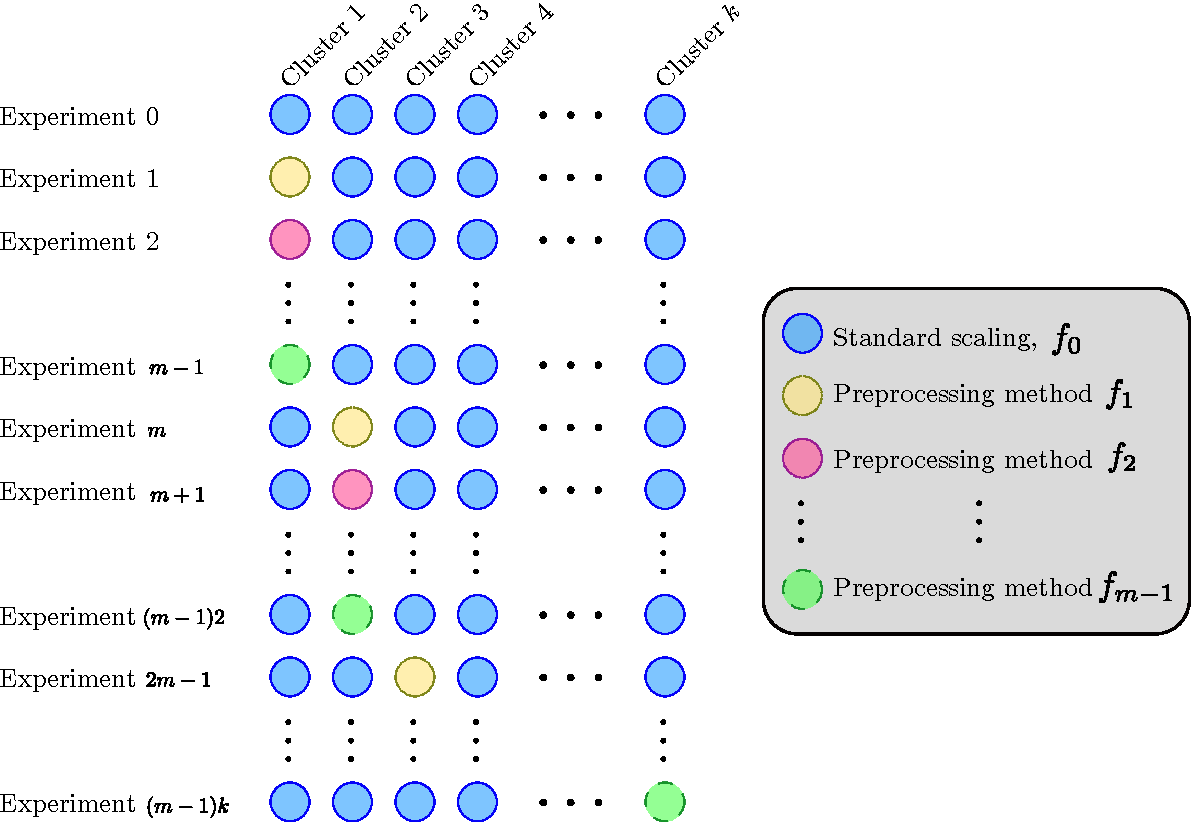
\includegraphics[width=\textwidth]{diagrams/prepmix-diagram.pdf}
    \end{center}
    \caption{Illustration of ``ablation studies'' done for finding the optimal preprocessing method
    for each cluster, as part of the \ac{PREPMIX-CAPS} routine.}
    \label{fig:prepmix}
    \vspace*{-15pt}
\end{figure}

The goal of the \ac{PREPMIX-CAPS} preprocessing approach is preprocessing the
data using the mixture of preprocessing technique that gives the best
performance according to some validation metric. Usually, this is the
validation loss of the neural network being trained. As such, to select which
of the $f_0, f_1,\dots,f_{m-1}$ preprocessing techniques to apply to each
cluster, we need train the model from scratch for each combination of
preprocessing technique applied, in order to get the final validation loss.
We refer to this as one \textit{experiment}.
Recall that after clustering, we have $k$ clusters of variables and $m$ different
preprocessing methods to consider for each cluster. Trying all of the possible
combinations would require performing $m^k$ experiments, which is
computationally infeasible for large $k$ or $m$, especially if model training
is slow. Instead, we iteratively look at the isolated effect each of the
different preprocessing techniques have on a particular cluster, and repeat
this $k$ times, similar to an ablation study. This process is illustrated in
\cref{fig:prepmix}. For the clusters not being
considered in a particular experiment, a baseline preprocessing technique such
as standard scaling is applied to that cluster, as this technique in general
works well for most datasets (citation needed). This scheme reduces the number
of experiments from $m^k$ to $(m-1)k+1$, as we also do one experiment where the
baseline preprocessing technique is applied to all clusters. The scheme is
illustrated in \cref{fig:prepmix}, where we picked standard scaling as the
baseline preprocessing technique.

After these $(m-1)k+1$ experiments have been run, and the final validation loss has been recorded
for each experiment, we can analyse the results to determine what mixture of preprocessing
techniques to use. With \cref{fig:prepmix} as reference, let $\mathcal{L}_{C_{i},f_j}$
denote the validation loss associated with the experiment where
preprocessing method $f_j$, with $j>0$, was applied to cluster $C_i$.
For $C_1,\dots,C_k$, the validation loss
$\mathcal{L}_{C_i,f_0}$ is the validation loss from experiment 0, that is, the baseline experiment.
Then, the preprocessing method for cluster $C_i$ in the final mixture
is set to be $f_{\widehat{j}}$, where
\begin{equation}
    \widehat{j}=\argmin_{0 \leq j < m}  \mathcal{L}_{C_i,f_j}.
\end{equation}
This way of selecting the overall mixture based on separate marginal improvements in performance
makes the assumption
that the marginal improvements are not dependent on how variables in a different cluster are
preprocessed.
% TODO: comment on validity of this assumption?

\subsubsection{Optimisations}%
\label{ssub:Optimisations}

The different experiments, as shown in \cref{fig:prepmix}, have no dependencies
between them and can thus be executed in parallel. This allows speeding up the
experiment running phase through parallel computation.
Before starting the experiments, the set of \acp{GPU}
to use has to be configured, which we denote as $\mathcal{I}_{\textrm{device IDs}}$.
The number of jobs
to run concurrently on each \ac{GPU} at any point in time, denoted $n_{\textrm{num. jobs}}$, must
also be specified.
To allow parallel computation, all the experiments---or jobs---were encapsulated in a Python
\texttt{threading.Thread} object. The jobs were then allocated to the \acp{GPU} in
$\mathcal{I}_{\textrm{device IDs}}$ in a \textit{round-robin} fashion, that is, allocate the first
job to the first \ac{GPU}, the second job to the second \ac{GPU}, etc., wrapping around to the first
\ac{GPU} once we reach the last \ac{GPU}. This is done until up to
$\# \mathcal{I}_{\textrm{device IDs}} \cdot n_{\textrm{num. jobs}}$ have been allocated and
set to start executing.
When these jobs finish, subsequent experiments are scheduled in a similar fashion
fashion. Unlike standard \textit{round-robin} scheduling, each job is run until completion instead
of switching while they execute.

% \subsection{Hyperparameters}%
% \label{sub:Hyperparameters}
%
% For my experiments, I used the following selection of preprocessing techniques:
% \begin{itemize}
%     \item Standard scaling \textit{with time- and dimension-axis}
%     \item Standard scaling \textit{across time}
%     \item Standard scaling followed by $\tanh(\cdot)$ \textit{with time- and dimension-axis}
%     \item Standard scaling followed by $\tanh(\cdot)$ \textit{across time}
%     \item Min-Max scaling to $[0,1]$ \textit{with time- and dimension-axis}
%     \item Min-Max scaling to $[0,1]$ \textit{across time}
% \end{itemize}
% This gives $m=6$. From hyperparameter tuning on $k$, also found $k=20$ for amex dataset
% (TODO: don't go into datasets yet...).
% For both clustering methods, the number of bins parameter, required for computing some of the
% statistics, as well as estimating the \ac{pdf} values required for estimating the
% \ac{KL-divergence} between the random variables, was set to be
% $n_{\textrm{num. bins}}=5000$. The number of clusters $k$ to use, was tuned using the specific
% dataset the \ac{PREPMIX-CAPS} method was applied to, which is described in section TODO.

% }}}

\section{Conclusion}% Conclusion
\label{sec:Conclusion}% {{{

We have now looked at three different novel preprocessing methods,
\ac{EDAIN}, \ac{EDAIN-KL}, and \ac{PREPMIX-CAPS}. The \ac{EDAIN} layer starts by applying
an adaptive outlier removal transformation, followed by an adaptive shift and scale operation,
and finally and adaptive power transform operation to reduce skewness. The layer also has
two modes, \textit{local-aware} and \textit{global-aware}, designed to handle highly
multimodal data and data with fewer modes, respectively. To optimise the parameters of
the \ac{EDAIN} layer, it is prepended to an existing neural network and the
\ac{EDAIN} parameters and neural network parameters are the simultaneously optimised using
stochastic gradient descent. We then looked at the \ac{EDAIN-KL} layer, which has the same
four sublayers as \ac{EDAIN}, but instead of optimising these using gradient descent, the layer
is treated as a bijector. Then it is optimized by minimizing the \ac{KL-divergence} between the
training data and a standard  normal distribution, transformed by the \ac{EDAIN-KL} layer.
After this, the training data is normalized by applying the inverse transformation.
The final method we looked at was the \ac{PREPMIX-CAPS} procedure, which is an automated
pipeline for selecting which static preprocessing technique to apply to each variable. It does this
by first clustering all the predictor variables. Then, through a parallel experiment
running phase, it selects the preprocessing method that minimizes the validation loss for each
cluster.

% }}}

%%%%%%%%%%%%%%%%%%%%%%%%%%%%%%%%%%%%%%%%%%%%%%%%%%
\chapter{Results} %%%%         Results        %%%%
%%%%%%%%%%%%%%%%%%%%%%%%%%%%%%%%%%%%%%%%%%%%%%%%%%

% TODO: introduction to this chapter

% Amex convergence plot (a) loss (b) AMEX metric
\begin{figure}[htp]
\centering
\begin{subfigure}[b]{0.99\textwidth}
    \centering
    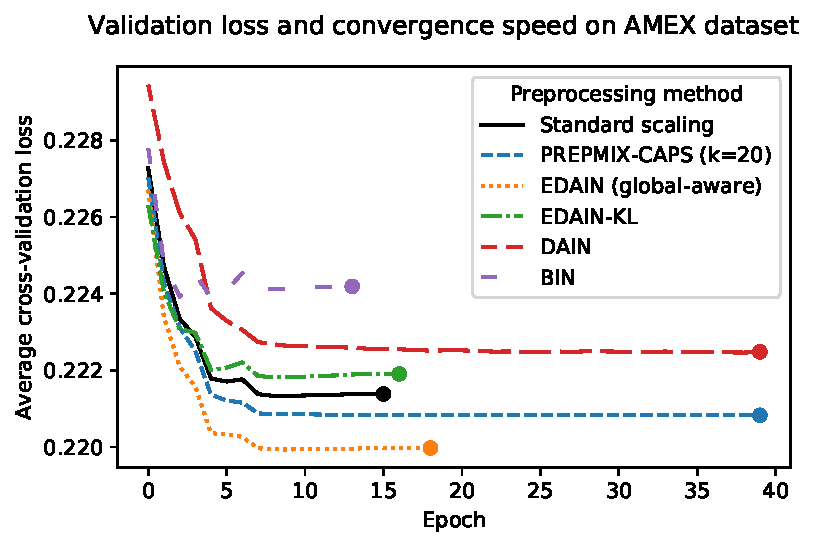
\includegraphics[width=\textwidth]{figures/amex_performance_convergence.pdf}
    \caption{Average cross-validation loss of \ac{RNN} model after each training epoch.
    Lower is better.}
    \label{fig:amex_performance_loss}
\end{subfigure}
\hfill
\begin{subfigure}[b]{0.99\textwidth}
    \centering
    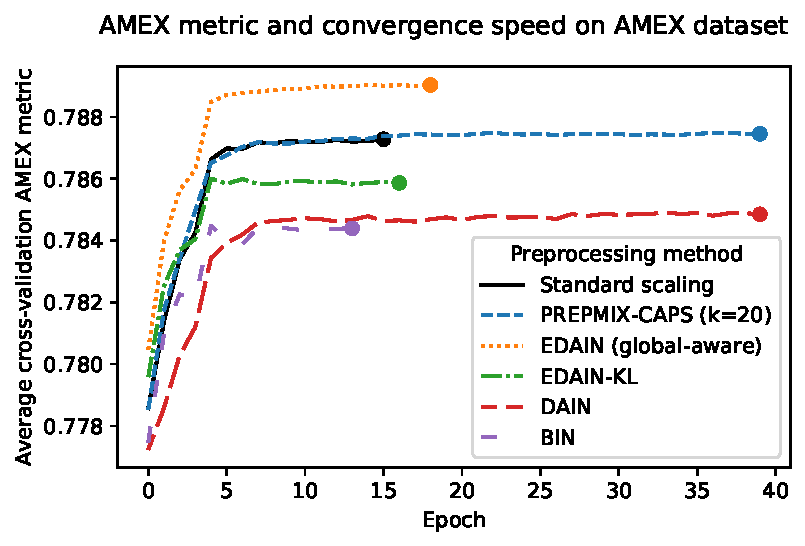
\includegraphics[width=\textwidth]{figures/amex_performance_convergence_metric.pdf}
    \caption{Average cross-validation American Express competition metric of the \ac{RNN} model
    after each training epoch. Higher is better.}
    \label{fig:amex_performance_metric}
\end{subfigure}
\caption{
    The plots show the average cross-validation performance of different preprocessing methods
    applied to the American Express dataset when training a \ac{RNN} binary classification model.
    The cross-validation was done using five disjoint 20\% validation sets.
    The dot highlights the earliest epoch where all five models are deemed to have converged by
    the early stopper, and can be interpreted as the convergence speed.
}%
\label{fig:amex_performance}
\end{figure}

% Amex performance table
\begin{table}[htp]
    \centering
    \begin{tabular}{lll}
        \toprule
        Method & Validation loss & AMEX metric \\
        \midrule
        Standard scaling & $0.2213 \pm 0.0039$ & $0.7872 \pm 0.0068$ \\
        PREPMIX-CAPS (k=20) & $0.2208 \pm 0.0033$ & $0.7875 \pm 0.0053$ \\
        EDAIN (global-aware) & $\mathbf{0.2199} \bm\pm \mathbf{0.0034}$ & $\mathbf{0.7890} \bm\pm \mathbf{0.0078}$ \\
        EDAIN-KL & $0.2218 \pm 0.0040$ & $0.7858 \pm 0.0060$ \\
        DAIN & $0.2224 \pm 0.0035$ & $0.7847 \pm 0.0054$ \\
        BIN & $0.2237 \pm 0.0038$ & $0.7829 \pm 0.0064$ \\
        \bottomrule
    \end{tabular}%
    \label{tab:amex_performance}%
    \caption{
        Evaluation results using the American Express default prediction dataset. Lower validation
        loss and higher AMEX metric is better.
        All confidence intervals are based on evaluation metrics from 5 cross-validation folds,
        and are asymptotic normal 95\% confidence intervals.
        The experiment methodology, including a description of the metrics,
        is described in  \cref{sec:amex_meth}.
}
\end{table}


% Amex fold breakdown
\begin{figure}[htp]
\begin{center}
    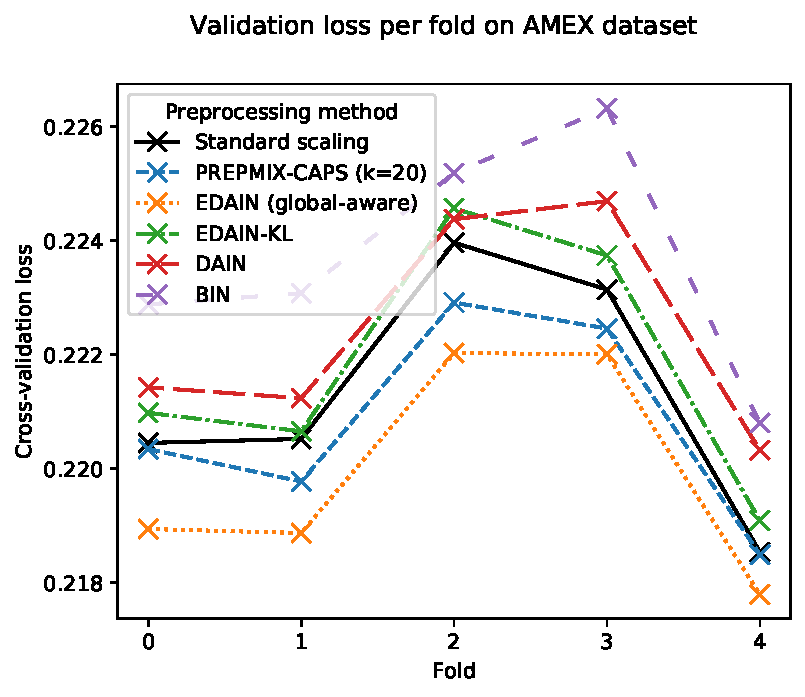
\includegraphics[scale=1]{figures/amex_performance_convergence_per_fold}
\end{center}
\caption{Validation loss at convergence for each of the five folds in the American Express
default prediction dataset.}
\label{fig:amex_folds}
\end{figure}


% LOB performance table
\begin{table}[htp]
    \centering
    \begin{tabular}{lll}
        \toprule
        Method & Cohen's Kappa, $\kappa$ & Average $F_1$-score \\
        \midrule
        Standard scaling & $0.2772 \pm 0.0550$ & $0.5047 \pm 0.0403$ \\
        Min-max scaling & $0.2618 \pm 0.0783$ & $0.4914 \pm 0.0603$ \\
        BIN & $0.3670 \pm 0.0640$ & $0.5889 \pm 0.0479$ \\
        DAIN & $0.3588 \pm 0.0506$ & $0.5776 \pm 0.0341$ \\
        EDAIN (local-aware) & $\bm{0.3836 \pm 0.0554}$ & $\bm{0.5946 \pm 0.0431}$ \\
        EDAIN (global-aware) & $0.2820 \pm 0.0706$ & $0.5111 \pm 0.0648$ \\
        EDAIN-KL & $0.2870 \pm 0.0642$ & $0.5104 \pm 0.0519$ \\
        \bottomrule
    \end{tabular}%
    \label{tab:lob_performance}%
    \caption{
        Evaluation results using the FI-2010 limit order book dataset..
        Higher $\kappa$ and higher $F_1$-score is better.
        All confidence intervals are based on evaluation metrics from 9 cross-validation folds,
        and are asymptotic normal 95\% confidence intervals.
        The experiment methodology, including a description of the metrics,
        is described in  \cref{sec:lob_meth}.
    }
\end{table}

% LOB cross-validation breakdown
\begin{figure}[htp]
\begin{center}
    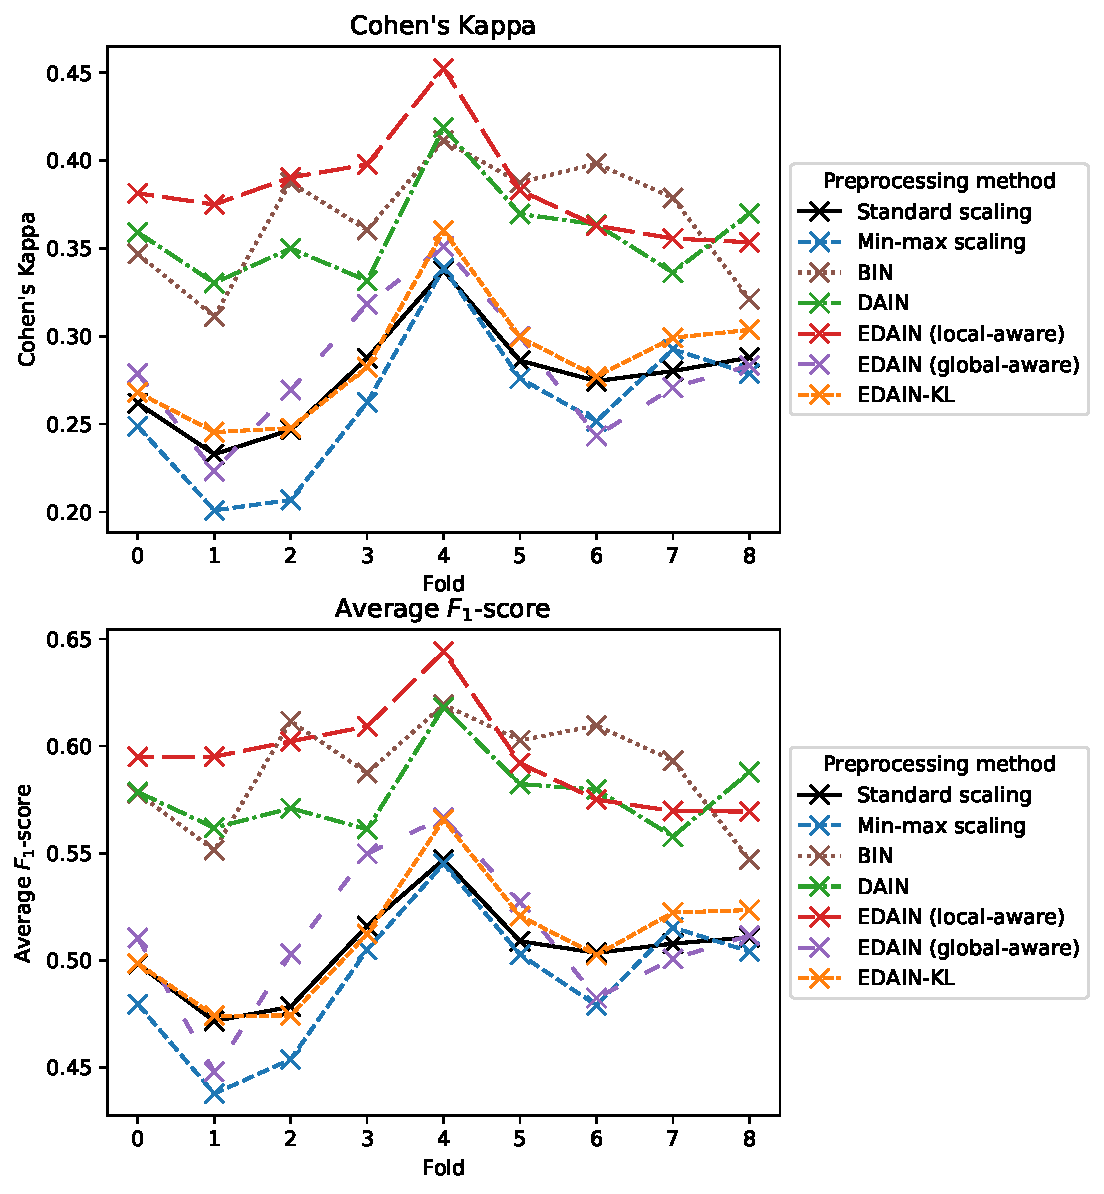
\includegraphics[width=\textwidth]{figures/lob_performance_per_fold.pdf}
\end{center}
\caption{Validation $\kappa$ and average $F_1$-value at convergence for each of the
    nine folds in the FI-2010 limit order book dataset.}
\label{fig:lob_folds}
\end{figure}


\clearpage

%%%%%%%%%%%%%%%%%%%%%%%%%%%%%%%%%%%%%%%%%%%%%%%%%%%%%%%%%%%%%
\section{Evaluation methodology}%%%  Evaluation methodology %%
\label{sec:Evaluation methodology}%%%%%%%%%%%%%%%%%%%%%%%%%%%%%

Small introduction

% Sequence model architecture
\subsection{Sequence model architecture}% {{{
\label{sub:Sequence model architecture}

% }}}

% Fitting the models
\subsection{Fitting the models}% {{{
\label{sub:Fitting the models}

Mention scheduling, early stopping, optimizer used, learning rate etc.
% }}}

% Tuning adaptive preprocessing model hyperparameters
\subsection{Tuning adaptive preprocessing model hyperparameters}% {{{
\label{sub:Tuning adaptive preprocessing model hyperparameters}

Details on the tuning for all the methods presented
% }}}

% Evaluation metric
\subsection{Evaluation metrics}% {{{
\label{sub:Evaluation metrics}

% }}}

% Cross-validaiton
\subsection{Cross-validation}% {{{
\label{sub:Cross-validation}

Mention both how cross-validation is done on American Express dataset, and how done differently
on Limit Order Book dataset.

% }}}

%%%%%%%%%%%%%%%%%%%%%%%%%%%%%%%%%%%%%%%%%%%%%%%%%%%
\section{Simulation study}%%%  Simulation study   %%
\label{sec:Simulation study}%%%%%%%%%%%%%%%%%%%%%%%%%

Small introduction, including motivation

% Multivariate time-series data generation algorithm
\subsection{Multivariate time-series data generation algorithm}% {{{
\label{sub:Multivariate time-series data generation algorithm}



% }}}

% Negative effects of irregularly-distributed data
\subsection{Negative effects of irregularly-distributed data}% {{{
\label{sub:Negative effects of irregularly-distributed data}


% }}}

% Preprocessing method experiments
\subsection{Preprocessing method experiments}% {{{
\label{sub:Preprocessing method experiments}



% }}}

%%%%%%%%%%%%%%%%%%%%%%%%%%%%%%%%%%%%%%%%%%%%%%%%%%%%%%%%%%%%%%%%%%%%%%%%
\section{American Express default prediction dataset}%%%  Amex dataset %%%
\label{sec:American Express default prediction dataset}%%%%%%%%%%%%%%%%%%%%

% Description
\subsection{Description}% {{{
\label{sub:Description}

% }}}

% Evaluation methodology
\subsection{Evaluation methodology}% {{{
\label{sec:amex_meth}

% }}}

% Preprocessing method experiments
\subsection{Preprocessing method experiments}% {{{
\label{sub:Preprocessing method experiments}



% }}}

%%%%%%%%%%%%%%%%%%%%%%%%%%%%%%%%%%%%%%%%%%%%%%%%%%%%%%%%%%%%%
\section{FI-2010 Limit order book dataset}%%%  LOB dataset %%%
\label{sec:American Express default prediction dataset}%%%%%%%%

% Description
\subsection{Description}% {{{
\label{sub:Description}

% }}}

% Evaluation methodology
\subsection{Evaluation methodology}% {{{
\label{sec:lob_meth}

% }}}

% Preprocessing method experiments
\subsection{Preprocessing method experiments}% {{{
\label{sub:Preprocessing method experiments}



% }}}

%%%%%%%%%%%%%%%%%%%%%%%%%%%%%%%%%%%%%%%%%%%%%%%%%%%
\chapter{Discussion} %%%%    Discussion        %%%%
%%%%%%%%%%%%%%%%%%%%%%%%%%%%%%%%%%%%%%%%%%%%%%%%%%%

% TODO: introduction to this chapter

% EDAIN
\section{EDAIN}% {{{
\label{sec:EDAIN-discuss}

% }}}

% EDAIN-KL
\section{EDAIN-KL}% {{{
\label{sec:EDAIN-KL-discuss}

% One advantage is that if DNN model changes, can still keep the bijector and just retransform
% the data later. Do not have to add overhead of adaptive layer like with EDAIN

% }}}

% PREPMIX-CAPS
\section{PREPMIX-CAPS}% {{{
\label{sec:PREPMIX-CAPS}


% }}}

%%%%%%%%%%%%%%%%%%%%%%%%%%%%%%%%%%%%%%%%%%%%%%%%%%
\chapter{Conclusion} %%%%     Conclusion      %%%%
%%%%%%%%%%%%%%%%%%%%%%%%%%%%%%%%%%%%%%%%%%%%%%%%%%

% Summary
\section{Summary}% {{{
\label{sec:Summary}



Conclusion goes here.



% }}}

% Main contributions
\section{Main contributions}% {{{
\label{sec:Main contributions}

% }}}


% Future work
\section{Future work}% {{{
\label{sec:Future work}

% }}}

% Appendix
% Appendix {{{
\clearpage
 %% reset page counter and start appendix pages with A
\pagenumbering{arabic}
\renewcommand*{\thepage}{A\arabic{page}}

%% Appendix goes here
%\appendix
%
%\chapter{Appendix title}
%
%Appendix goes here.

% }}}

% References {{{
%%References part of appendices
% References: modify the file refs.bib
\bibliographystyle{plainnat}
\bibliography{refs}


% }}}
\end{document}
% vim: set foldmethod=marker:
